\documentclass[11pt, oneside]{article}   	% use "amsart" instead of "article" for AMSLaTeX format
\usepackage[margin=2.25cm]{geometry}                		% See geometry.pdf to learn the layout options. There are lots.
\geometry{letterpaper}                   		% ... or a4paper or a5paper or ... 
%\geometry{landscape}                		% Activate for rotated page geometry
%\usepackage[parfill]{parskip}    		% Activate to begin paragraphs with an empty line rather than an indent
\usepackage{graphicx}				% Use pdf, png, jpg, or eps§ with pdflatex; use eps in DVI mode
								% TeX will automatically convert eps --> pdf in pdflatex	
								
%\usepackage[T1]{fontenc}
%\usepackage[utf8]{inputenc}
%\usepackage{babel}
%\usepackage{csquotes}
									
\usepackage{amssymb}
\usepackage{lineno}
\usepackage{authblk}
\usepackage{hyperref}
\usepackage{xcolor}

\usepackage{natbib}

\hypersetup{
    colorlinks,
    linkcolor={red!50!black},
    citecolor={blue!50!black},
    urlcolor={blue!80!black}
}

\linenumbers


\author{Joseph D. Hughes}
\affil{U.S. Geological Survey, Model Support and Maintence Branch, 927 W Belle Plaine Ave, Chicago, IL, USA}
\author{Christian D. Langevin}
\affil{U.S. Geological Survey, Model Support and Maintence Branch, 2280 Woodale Dr, Mounds View, MN, USA}
\author{Scott R. Paulinski}
\affil{U.S. Geological Survey, California Water Science Center, 4165 Spruance Road, Suite 200, San Diego, CA, USA}
\author{Joshua D. Larsen}
\affil{U.S. Geological Survey, California Water Science Center, 6000 J Street, Placer Hall, Sacramento, CA, USA}
\author{David Brakenhoff}
\affil{Artesia Water, Korte Weistraat 12, Schoonhoven, Netherlands}


\begin{document}
\onecolumn

\title{Modern and Reproducible Groundwater Modeling Workflows with FloPy} 

\maketitle


\begin{abstract}

%%% Leave the Abstract empty if your article does not require one, please see the Summary Table for full details.
\section{}
For full guidelines regarding your manuscript please refer to \href{http://www.frontiersin.org/about/AuthorGuidelines}{Author Guidelines}.

As a primary goal, the abstract should render the general significance and conceptual advance of the work clearly accessible to a broad readership. References should not be cited in the abstract. Leave the Abstract empty if your article does not require one, please see \href{http://www.frontiersin.org/about/AuthorGuidelines#SummaryTable}{Summary Table} for details according to article type. 


\end{abstract}

\section{Introduction}
%For Original Research Articles \citep{conference}, Clinical Trial Articles \citep{article}, and Technology Reports \citep{patent}, the introduction should be succinct, with no subheadings \citep{book}. For Case Reports the Introduction should include symptoms at presentation \citep{chapter}, physical exams and lab results \citep{dataset}.


FloPy is a popular Python package for constructing, running, and post processing MODFLOW-based groundwater models.  It is open source and developed with input from a growing community of modelers.  

It has been recommended as one way to facilitate repeatable research and sharing of ideas \citep{fienen2016}

We have FloPy to be particularly useful for teaching.  Annotated Jupyter notebooks, comparison with analytical solutions, ...

We rely on FloPy for MODFLOW development.  We write tests that rely on FloPy to construct and run models, and then read output.  We then verify that the output is as expected, by using the results from an analytical solution, results from another model, or results that have been confirmed to be correct.

We use FloPy to load models

 FloPy is used to pioneer new methods and analysis tools, such as deep learning approaches for improving groundwater model calibration \citep{sun2018, zhou2021}, regionalization of residence times using metamodeling \citep{starn2018}, iterative ensemble approaches for calibration and uncertainty quantification \citep{white2018ies}, and exploration of alternative parameterization schemes for risk analysis \citep{knowling2019}. There are numerous examples of constructing MODFLOW models to solve applied groundwater problems \citep{befus2017, vanengelen2018, ebeling2019, zipper2019, befus2020}.  Used in GIS-based tools, such as FREEWAT \citep{freewat2018} and other cyberinfrastructures \citep{essawy2018} to export models into MODFLOW datasets.  FloPy can also be used as the ``glue'' to help couple MODFLOW to other hydrological models \citep{burek2020} or even to agent-based models designed to quantify the effects of decision makers on environmental behavior \citep{jaxarozen2019}. 

\cite{bakker2016scripting} describe the general approach for working with models within the python environment and emphasize the reproducible nature of developing models through scripting.  FloPy has continued to advance since it was first described by \cite{bakker2016scripting}.  The purpose of this paper is to highlight some of these important advances, provide examples that demonstrate these new capabilities, and reinforce the advantages of the modern scripting workflow for developing reproducible groundwater models that can be easily updated as new data become available.  The important advances described here can be summarized as

\begin{itemize}
\item expanded support for MODFLOW-2005, MODFLOW-NWT, MODFLOW-LGR, MODFLOW-USG, SEAWAT, MT3D, MT3D-USGS
\item rapid and robust support for all MODFLOW 6 models, packages, and options,
\item generalized support for structured and unstructured model grids,
\item implementation of new geoprocessing capabilities to rapidly populate models with data, 
\item export capabilities for writing model data to a variety of output formats, 
\item plotting capabilities for map and cross-section views of model data, and
\item simplified access to model results.
\end{itemize}


\section{FloPy Support for MODFLOW 6}

The most recent version of MODFLOW (MODFLOW 6) is an object-oriented program and framework developed to provide a platform for supporting multiple models and multiple types of models within the same simulation \citep{modflow6gwf, modflow6framework, morway2021use}. These models can be independent of one another with no interaction, they can exchange information, or they can be tightly coupled at the matrix level by adding them to the same numerical solution. Transfer of information between models is isolated to exchange objects, which allow models to be developed and used independently. Within this new framework, a regional-scale groundwater model may be coupled with multiple local-scale groundwater models. 

MODFLOW 6 currently includes the Groundwater Flow (GWF) Model and the Groundwater Transport (GWT) Model each with packages to represent surface water processes,  groundwater extraction, external boundaries, mass sources and sinks, and mass sorption and reactions.  GWF and GWT models can be developed using regular model grids consisting of layers, rows, and columns or they can be developed using more general unstructured grids using many of the concepts and numerical approaches available in MODFLOW-USG  \citep{modflowusg}.  MODFLOW 6 also includes advanced formulations to simulate three-dimensional anisotropy and dispersion \citep{modflow6xt3d}, coupled variable-density groundwater flow and transport \citep{langevin2020hydraulic}, and a water mover package to represent natural and managed hydrologic connections \citep{morway2021use}.

Development and testing of the MODFLOW 6 program relies heavily on tight integration with FloPy.  A key component of this tight integration is the capability to quickly support new MODFLOW 6 models and packages with FloPy.  Unlike the FloPy support for previous MODFLOW versions (for example, MODFLOW-2005, MODFLOW-NWT, MODFLOW-USG, and SEAWAT), the FloPy python classes for MODFLOW 6 are dynamically generated from simple text files that describe the input file structure.  This allows MODFLOW 6 developers to write tests for new models, packages, and functionality as they are developed.  All MODFLOW 6 model input files are described using ``definition files.''  These definition files are used to generate the user input and output guide.  These same definition files are also used to generate FloPy classes, with argument docstrings corresponding to input variable descriptions in the input and output guide.

\begin{figure}[h!]
	\begin{center}
		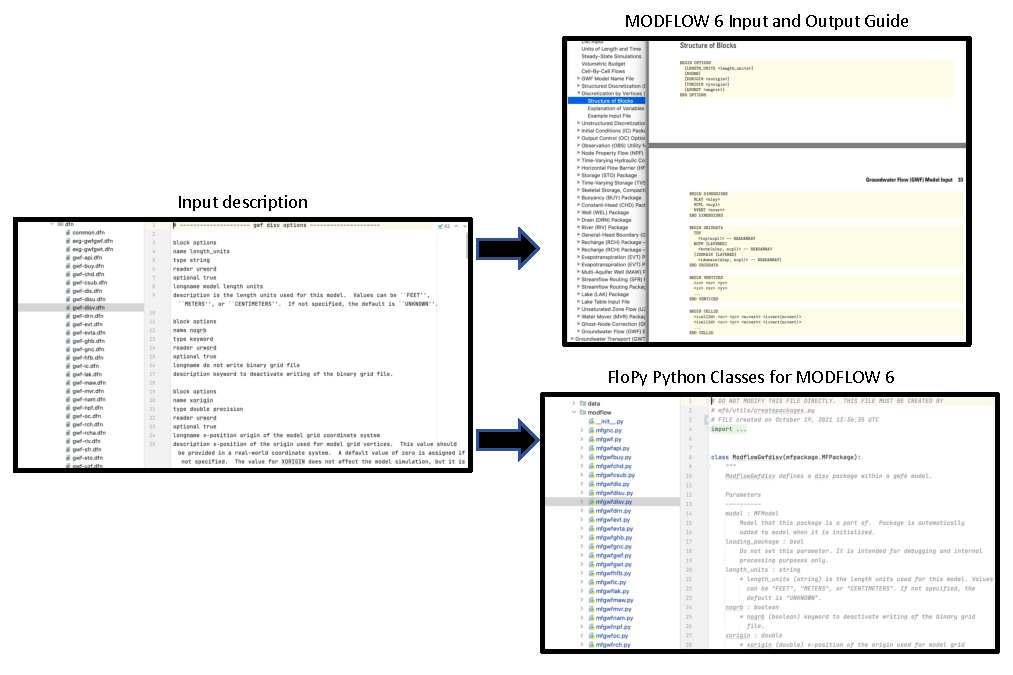
\includegraphics{figures/mf6definition.pdf}
	\end{center}
	\caption{Relation between MODFLOW 6 input description files and the MODFLOW 6 input and output guide and the FloPy Python classes for MODFLOW 6.}
	\label{fig:mf6definition}
\end{figure}


\section{Common Modeling Tasks}

\subsection{Generating Grids}

Support for a variety of different structured and unstructured grid types has been a recent focus of MODFLOW development \citep{modflowusg, modflow6gwf, modflow6xt3d}.  FloPy has been updated to support processing of different types of grids, such as those shown in figure \ref{fig:grids} through implementation of several different grid classes.  The regular MODFLOW grid consisting of layers, rows, and columns, continues to be a popular type of MODFLOW grid.  Regular MODFLOW grids can have constant row and column spacings, as shown in Figure \ref{fig:grids}A, or they can have variable row and column spacings to focus resolution around an area of interest, as shown in Figure \ref{fig:grids}B.  FloPy internally represents this type of grid as a StructuredGrid object.  

Nested grid \citep{modflowlgr2}
quadtree grid refinement \citep{gridgen}; 
then cite triangle \citep{trianglemesh} and 
then cite voronoi grid \citep{2020SciPy-NMeth} cite any groundwater papers? algomesh?).

FloPy gridding allows for innovation; mention Central Sands and the ability to simulate local-scale detail and regional-scale influence in the same simulation?

\begin{figure}[ht!]
\begin{center}
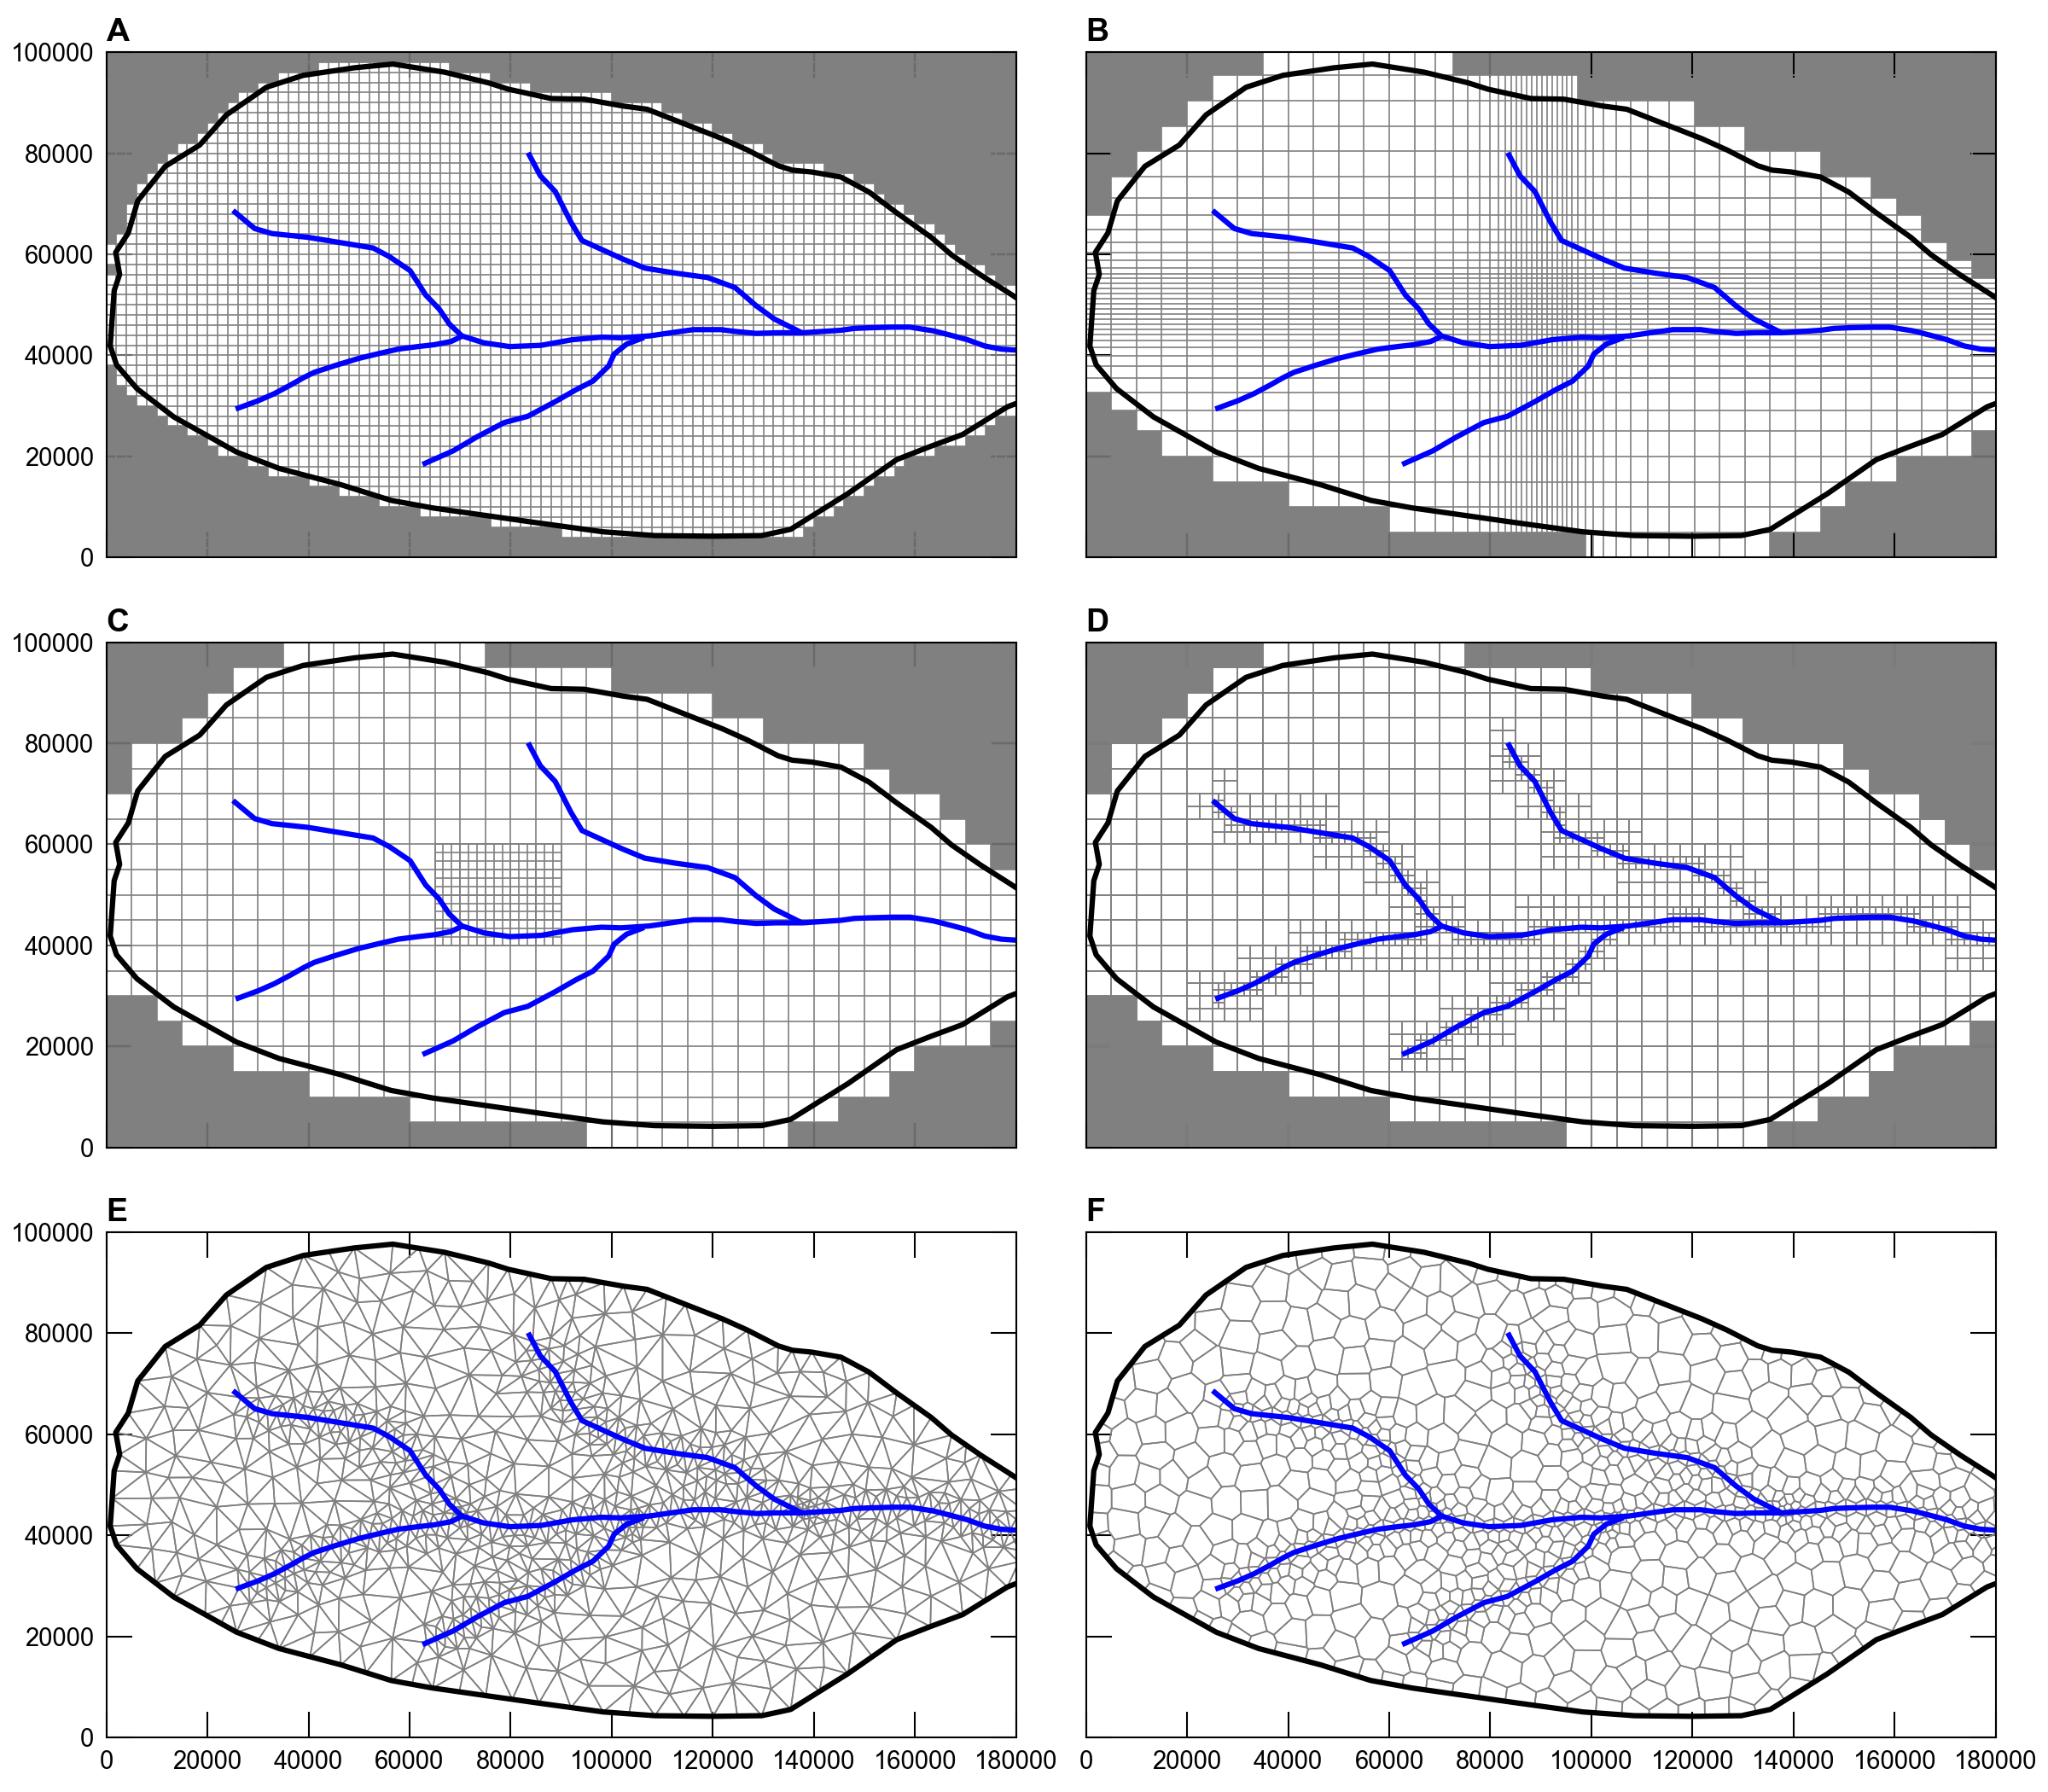
\includegraphics{figures/grids.png}
\end{center}
\caption{Examples of grids that can be generated and processed using FloPy for a hypothetical watershed, including (A) a regular structured MODFLOW grid, (B) a structured MODFLOW grid with irregular spacing, (C) a regular MODFLOW child grid nested within a regular MODFLOW parent grid, (D) a quadtree grid, (D) a triangular grid, and (E) a voronoi grid}\label{fig:grids}
\end{figure}


\subsection{Geospatial Processing}

Intersections, raster resampling, ...

\begin{figure}[ht!]
	\begin{center}
		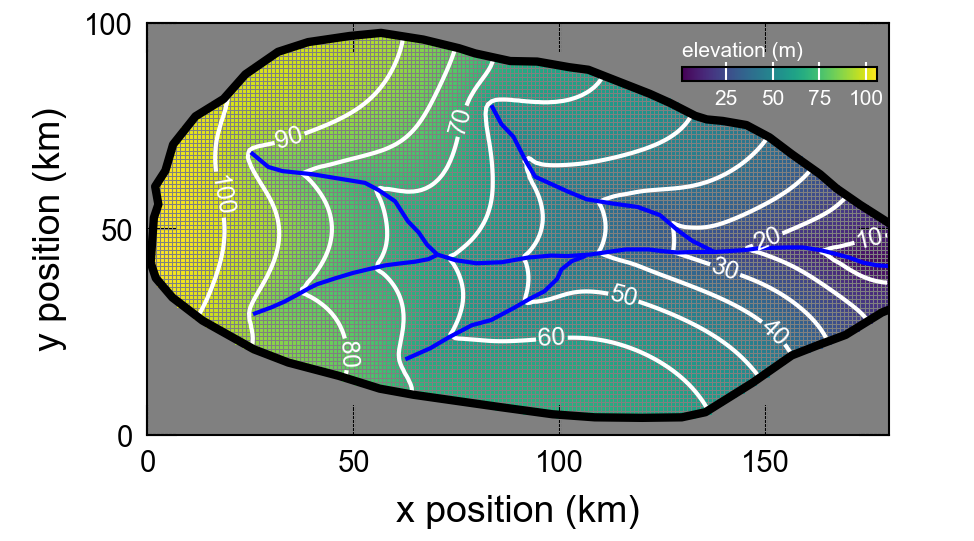
\includegraphics{figures/fine_topo.png}
	\end{center}
	\caption{High resolution digital elevation model of a hypothetical watershed.}
	\label{fig:dem}
\end{figure}

\begin{figure}[ht!]
	\begin{center}
		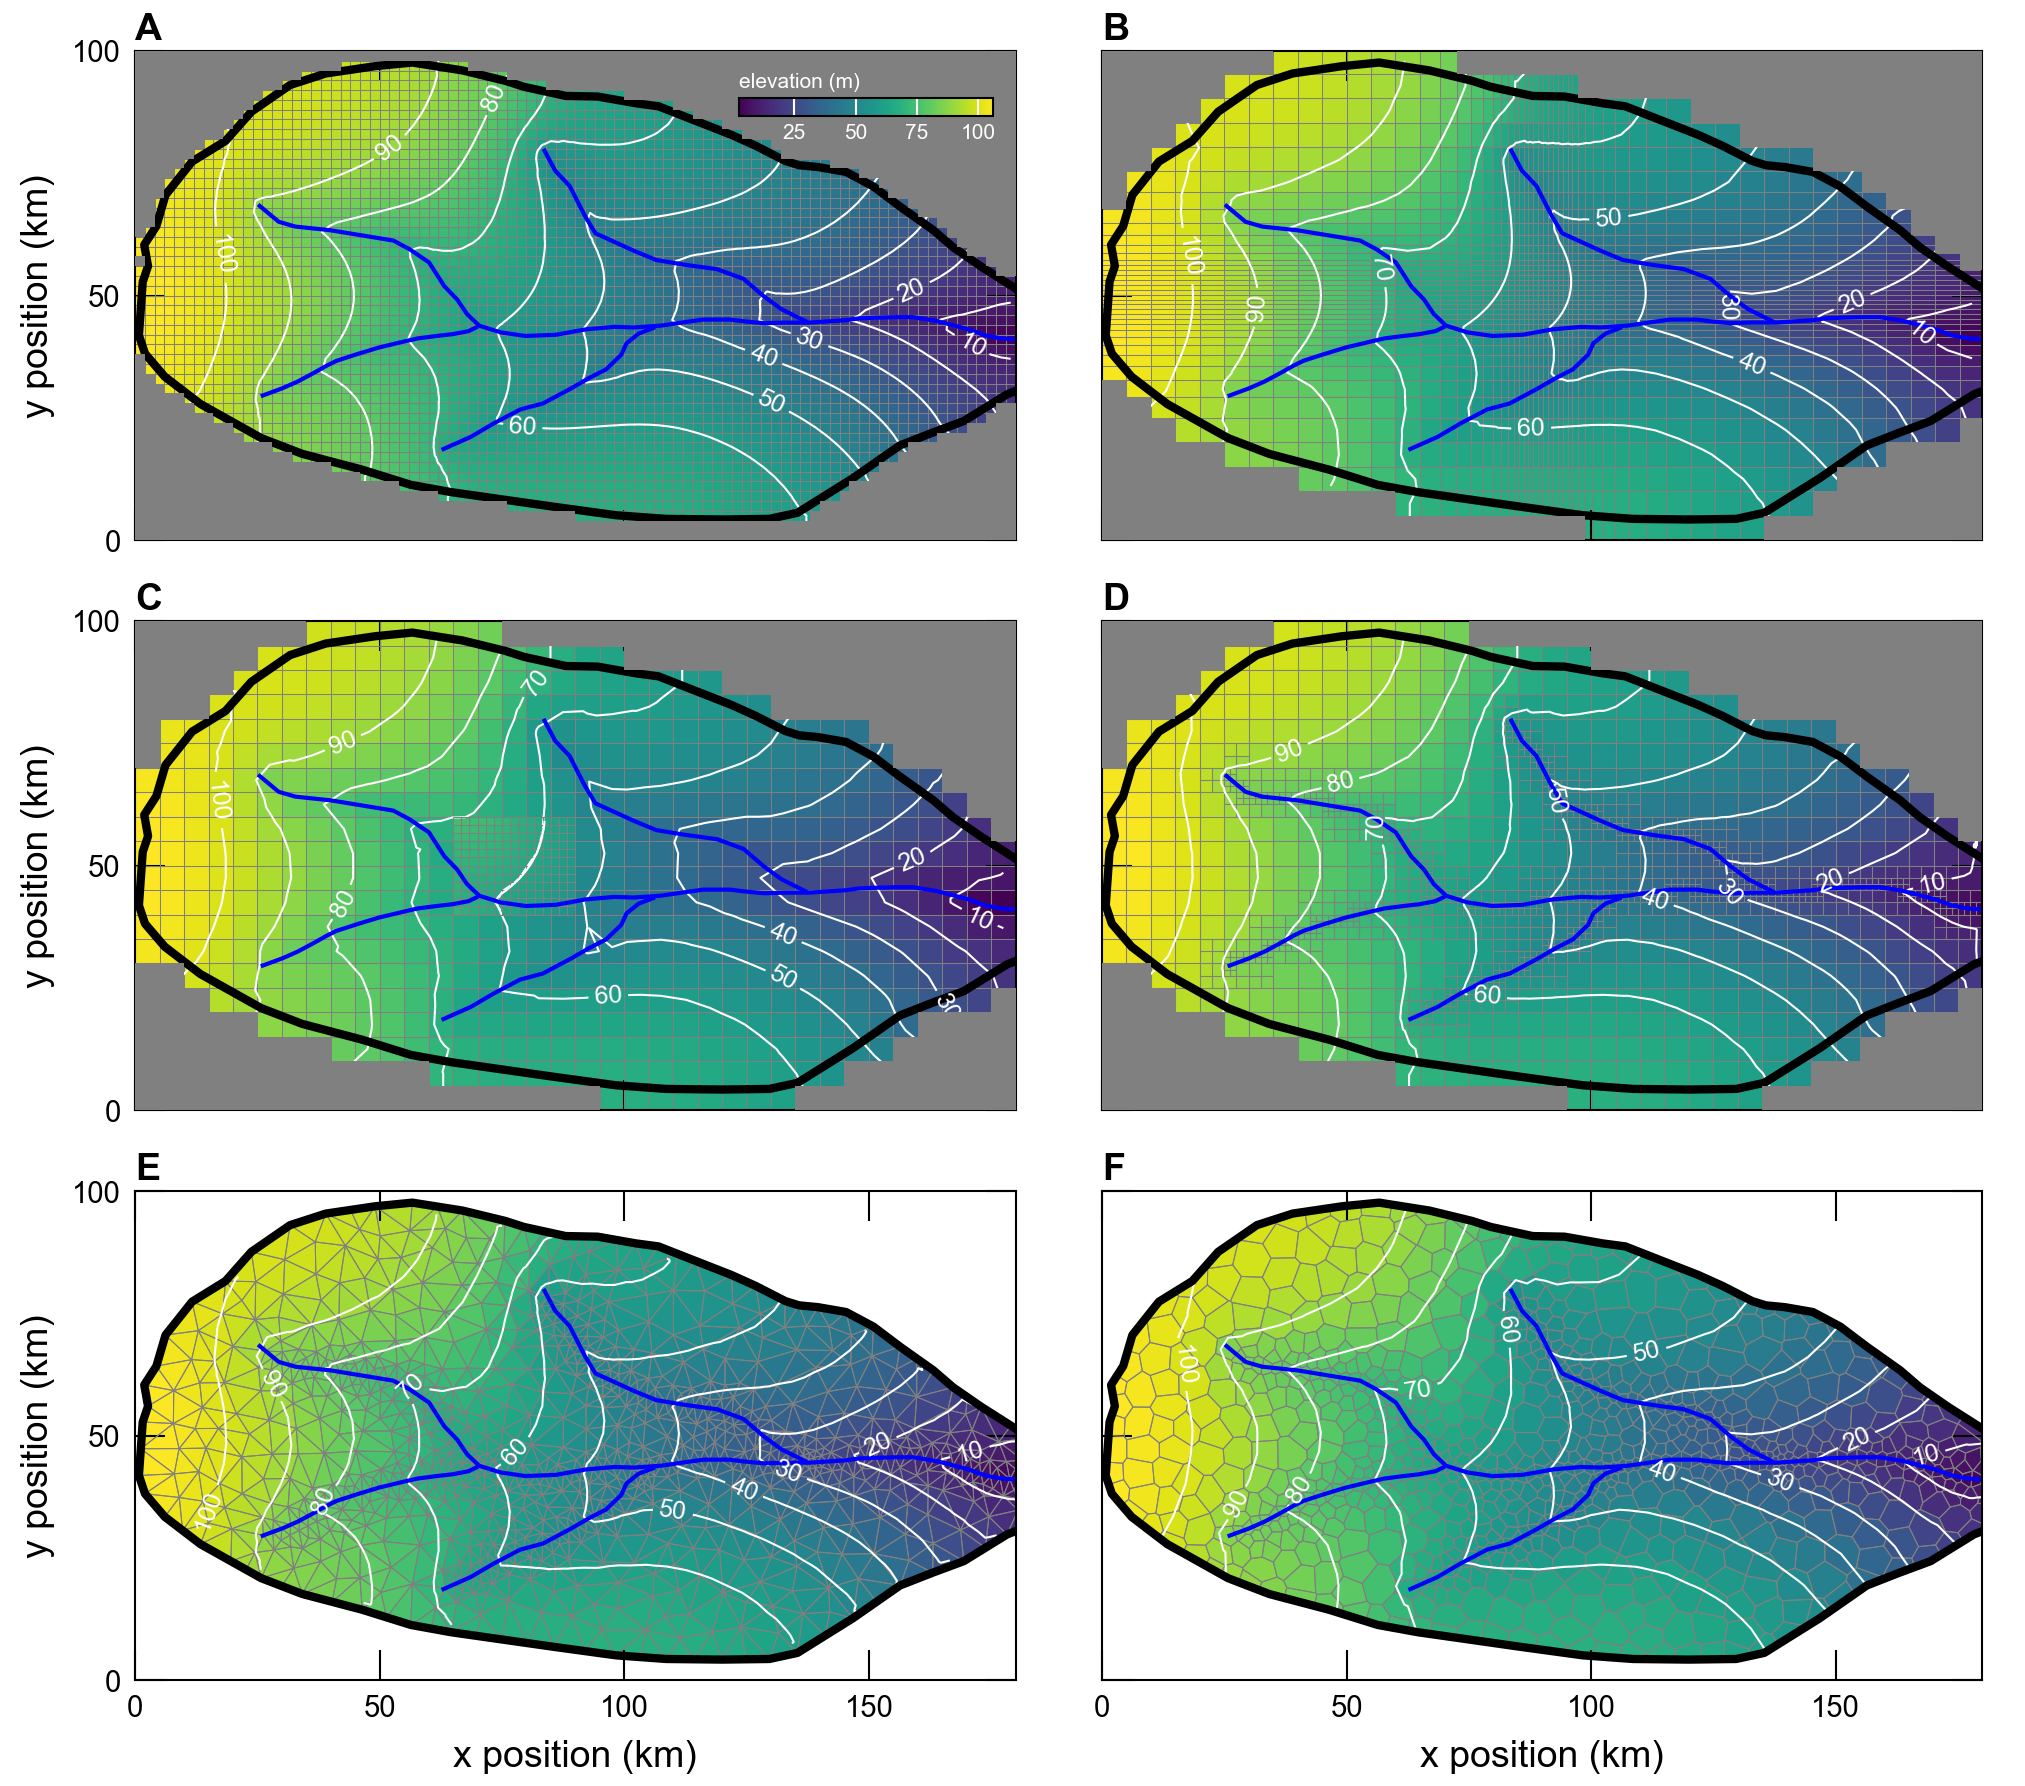
\includegraphics{figures/grids_geoprocessing.png}
	\end{center}
	\caption{Examples of the high resolution digital elevation model shown in figure~\ref{fig:dem} resampled on MODFLOW grids shown in figure~\ref{fig:grids} using FloPy, including (A) a regular structured MODFLOW grid, (B) a structured MODFLOW grid with irregular spacing, (C) a regular MODFLOW child grid nested within a regular MODFLOW parent grid, (D) a quadtree grid, (D) a triangular grid, and (E) a voronoi grid.}
	\label{fig:geoprocessing}
\end{figure}

\begin{figure}[ht!]
	\begin{center}
		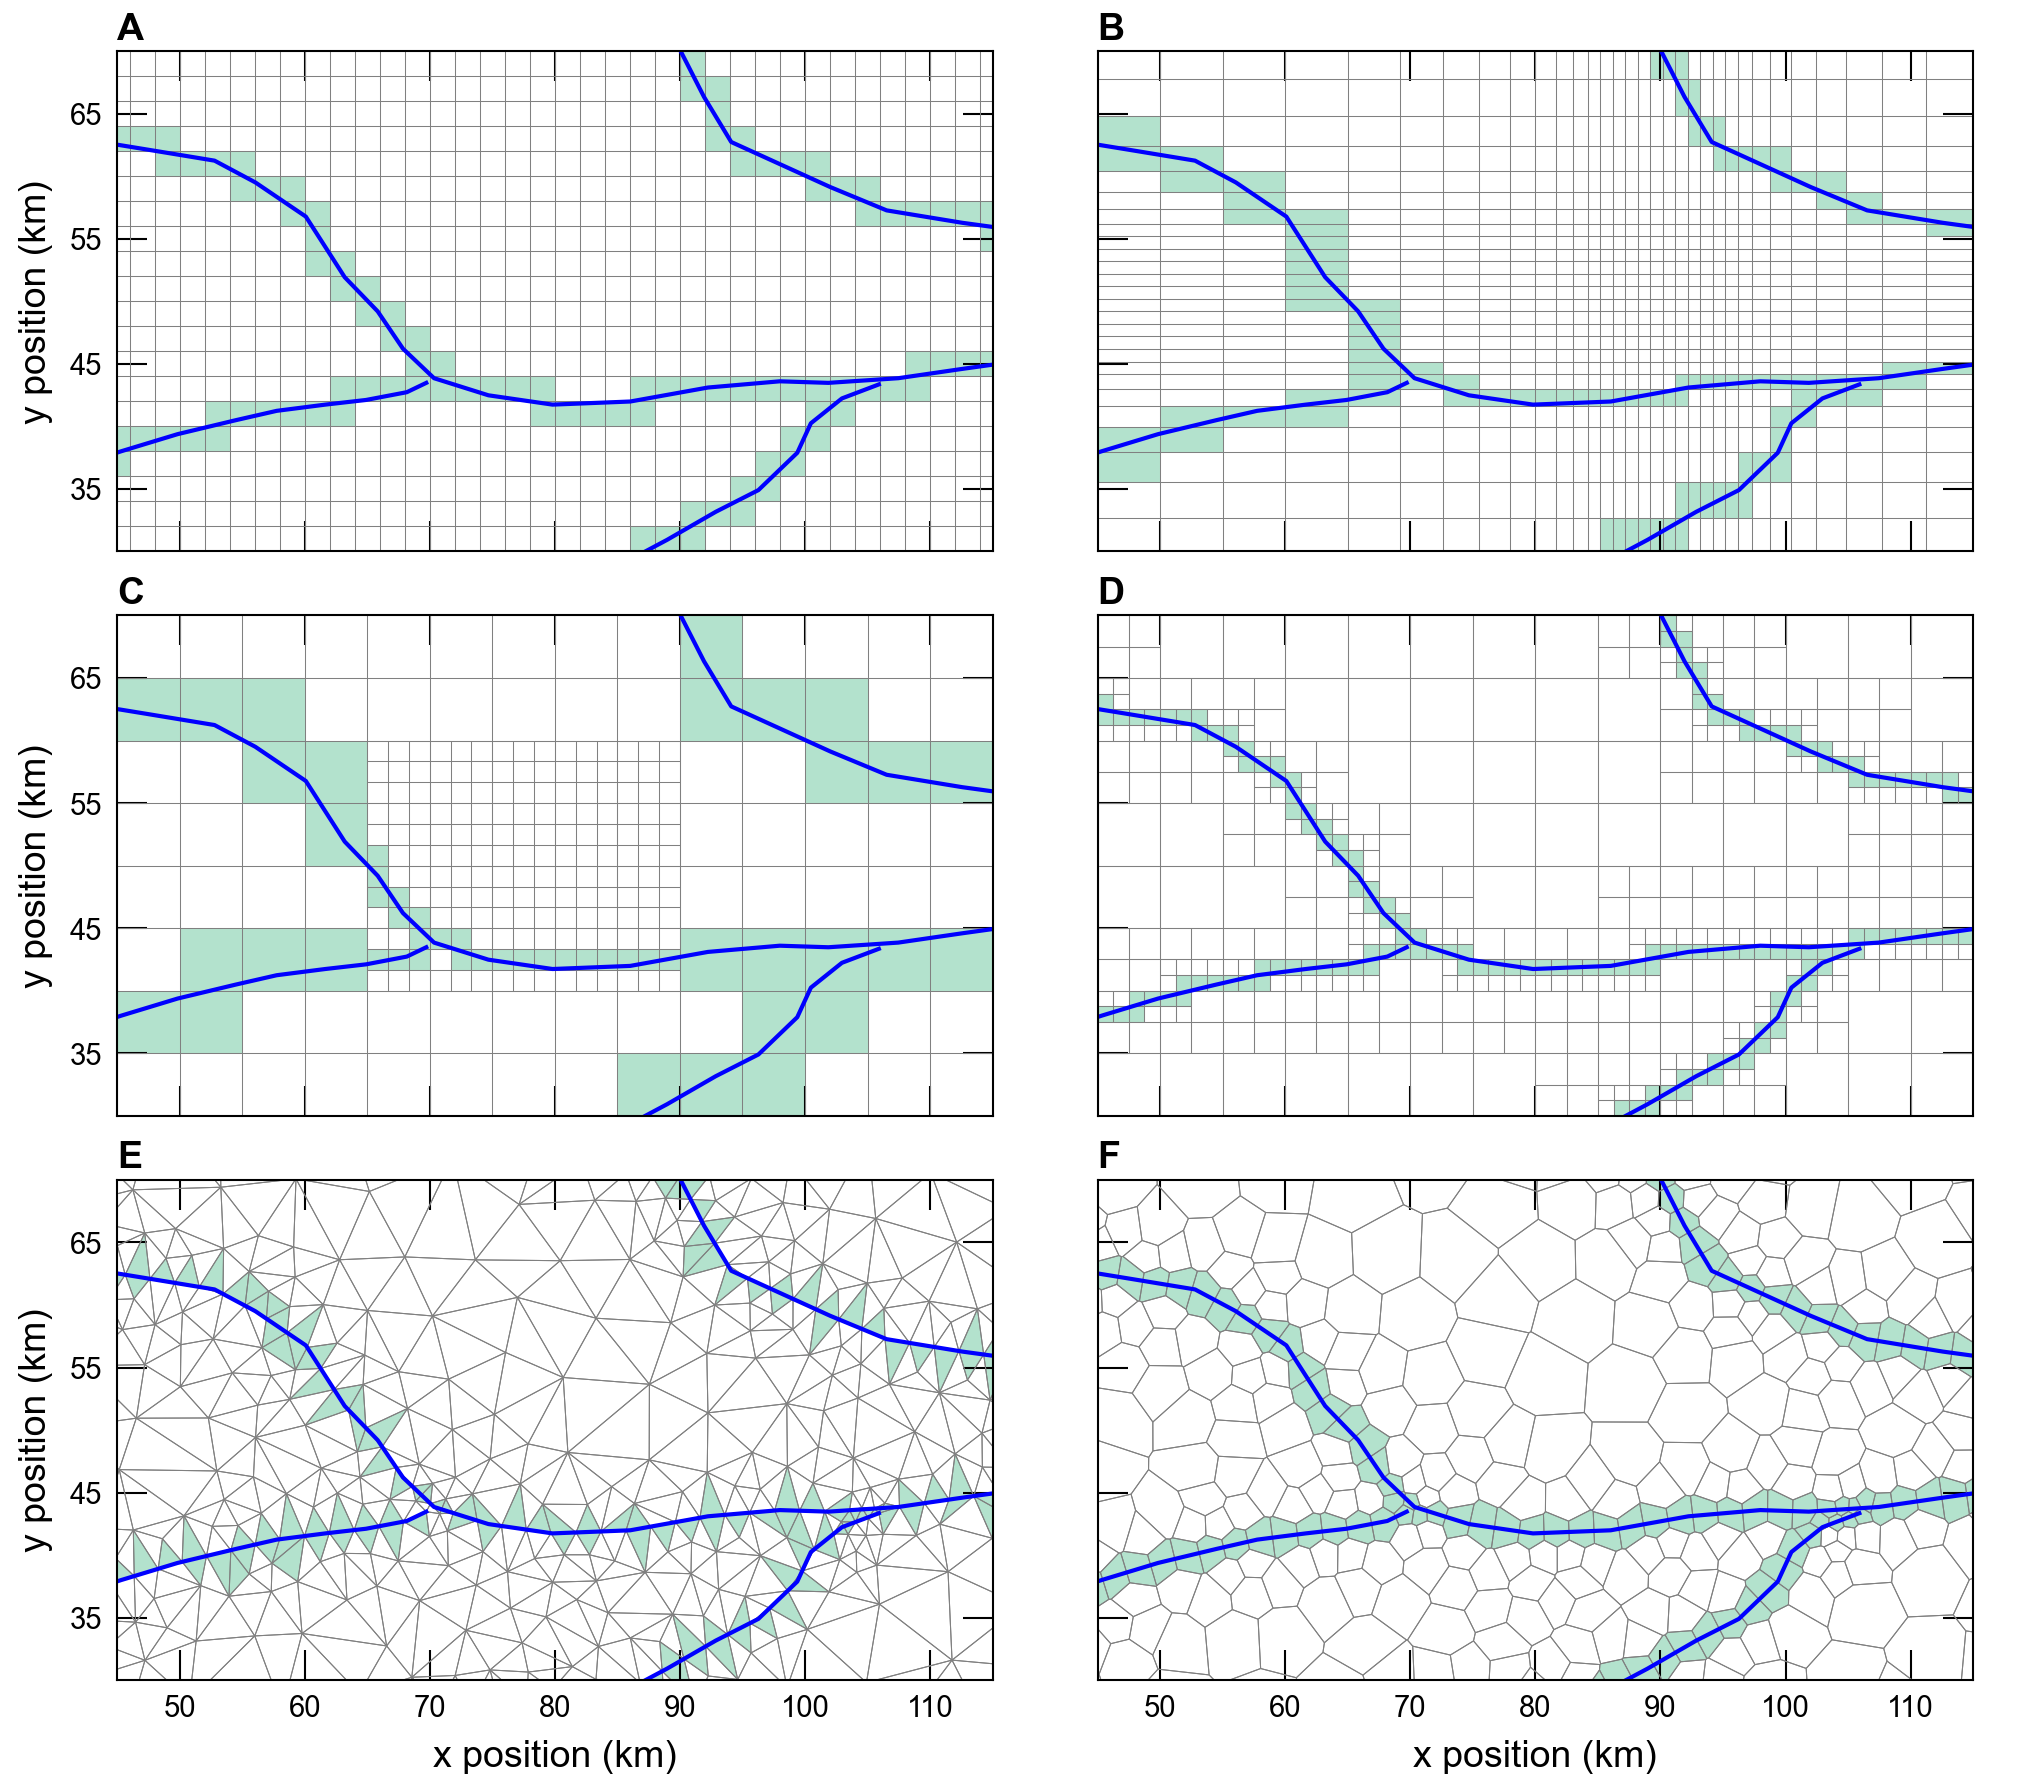
\includegraphics{figures/grids_intersection.png}
	\end{center}
	\caption{Examples of the intersection of a linear stream network and MODFLOW grids shown in figure~\ref{fig:grids} using FloPy, including (A) a regular structured MODFLOW grid, (B) a structured MODFLOW grid with irregular spacing, (C) a regular MODFLOW child grid nested within a regular MODFLOW parent grid, (D) a quadtree grid, (D) a triangular grid, and (E) a voronoi grid. The shaded cells represent cells that intersect the river network. The plots are centered on the location of the child grid shown in figure~\ref{fig:grids}C.}
	\label{fig:intersections}
\end{figure}


\subsection{Plotting}

\subsection{Exporting Grid Data to Other Formats}

shapefiles (all grids), VTK (all grids) and NetCDF (structured grids)

\section{Example}

Background of the McDonald Valley

\section{Discussion and Conclusions}
FloPy is a popular python package for building, running, and post processing groundwater models.  It is open source and developed with input from a growing community of modelers.  

Key findings

\begin{itemize}
\item FloPy fully supports creation and loading of all MODFLOW 6 models and packages.  FloPy classes can be built and updated automatically using MODFLOW 6 definition files, which describe input format.  FloPy also supports MODFLOW-2005, MODFLOW-NWT, MODFLOW-USG, MT3D, and MT3D-USGS.
\item FloPy contains a low-level Grid class, which can be used to represent regular MODFLOW grids consisting of layers, rows, and columns, or unstructured grids consisting of vertices and incidence lists.  The Grid class is used systemically throughout FloPy for geospatial operations, plotting, and exporting model information to supported formats.
\item Geospatial intersections of points, lines, and polygons with model grids and raster resampling onto model grids are common steps in model construction.  FloPy fully supports these geospatial operations through its grid intersection and raster resampling routines.  
\item Map and cross section plotting
\item Export to shapefiles, VTK, and NetCDF
\end{itemize}


\section*{Acknowledgments}
This is a short text to acknowledge the contributions of specific colleagues, institutions, or agencies that aided the efforts of the authors.

\section*{Supplemental Data}
 \href{http://home.frontiersin.org/about/author-guidelines#SupplementaryMaterial}{Supplementary Material} should be uploaded separately on submission, if there are Supplementary Figures, please include the caption in the same file as the figure. LaTeX Supplementary Material templates can be found in the Frontiers LaTeX folder.

\section*{Data Availability Statement}
The datasets [GENERATED/ANALYZED] for this study can be found in the [NAME OF REPOSITORY] [LINK].
% Please see the availability of data guidelines for more information, at https://www.frontiersin.org/about/author-guidelines#AvailabilityofData

\bibliographystyle{apalike} 
\bibliography{flopy}


\end{document}
